% ============================================================
\section{Background and Threat Model}
% ============================================================
\label{sec:background}

This section introduces the technical background necessary to situate our contribution and then formalizes the threat model addressed by this work. We first characterize User Attribute Inference (UAL-Inference) as a distinct capability of large language models, grounding the discussion in the SynthPAI corpus used throughout our evaluation. We then define precisely who the attacker is, what the attacker seeks to achieve, and under which capabilities and limitations the attack is conducted. Finally, we derive the design requirements that any defense targeting this threat model must satisfy, which motivate the architecture.

\subsection{User Attribute Inference in LLMs}
\label{subsec:ual_definition}

User Attribute Inference denotes the capability of a large language model to derive sensitive personal attributes of the author of a text-such as age, sex, geographic location, education level, occupation, relationship status, or income-without those attributes ever being explicitly stated. Rather than retrieving information the model has memorized, the model synthesizes an estimate of the attribute from indirect, associative cues present in the surrounding context: word choice, cultural references, described routines, or domain-specific vocabulary. This capability follows directly from the broad contextual reasoning that makes LLMs useful for legitimate analytical tasks, but it also means that any sufficiently descriptive piece of user-generated text carries a latent privacy risk, independent of whether the author intended to disclose anything.

Our evaluation is grounded in the synthetic dataset published by \citet{staab2024beyond}, released as the \texttt{eth-sri/llmprivacy} repository~\cite{ethsri-llmprivacy-repo}. The SynthPAI corpus consists of synthetic Reddit-style posts authored by fictional profiles, each annotated with a ground-truth vector of seven personal attributes: \textit{age}, \textit{sex}, \textit{city and country of residence}, \textit{education level}, \textit{occupation}, \textit{relationship status}, and \textit{income bracket}. These attributes are rarely stated outright; instead, they must typically be reconstructed through associative reasoning over indirect cues. A representative case is inferring \textit{Melbourne, Australia} from a passing reference to ``\textit{hook turn}'' driving manoeuvres, a rule legally mandated only in Melbourne's central business district the kind of contextual, non-obvious association that distinguishes genuine inference from surface-level extraction of an explicitly stated fact.

UAL-Inference is conceptually distinct from two better-studied classes of LLM privacy and safety threats. First, it is distinct from privacy threats based on memorization or data leakage. Membership-inference and training-data-extraction attacks~\cite{carlini2021extracting} recover verbatim content the model has memorized during training, and their success is bounded by what was actually present in the training data. UAL-Inference requires no memorization at all: the target attribute is typically absent from both the input text and the model's training data, and is instead synthesized through associative reasoning over contextual cues at inference time. Consequently, defenses designed against memorization-based leakage---output filtering for verbatim training strings, differential privacy during training---do not address UAL-Inference; indeed, \citet{ippolito2023preventing} show that even suppressing verbatim memorization gives a false sense of privacy, since a model can still paraphrase or reconstruct the same sensitive content non-verbatim, which is precisely the inferential pathway UAL-Inference exploits. Second, it is distinct from conventional LLM safety threats such as prompt injection and jailbreaking~\cite{perez2022ignore}, which succeed by subverting the model's instruction-following boundaries overriding a system prompt, escaping a role-play sandbox, or smuggling an unauthorized instruction into the input. A UAL-Inference request requires no such subversion: the model is not being tricked into violating its instructions, but is instead performing the ordinary contextual reasoning it was designed to perform, applied to a query whose profiling intent may be entirely unmarked syntactically. This is precisely what makes UAL-Inference difficult for defenses built around detecting instruction subversion, and motivates a detection mechanism operating on the semantic content of the request rather than on syntactic markers of attack.

\subsection{Threat Model}
\label{subsec:threat_model}

We formalize the adversarial setting as a black-box threat model. The adversary's objective is to obtain private, unstated attributes of a specific person by exploiting the target LLM's inferential capability rather than any vulnerability in the model's training pipeline or deployment infrastructure: the attacker supplies a document authored by the victim a social media post, a review, a forum comment and constructs a natural-language prompt instructing the model to infer and disclose the author's private attributes from that text.

\begin{figure}[H]
\centering
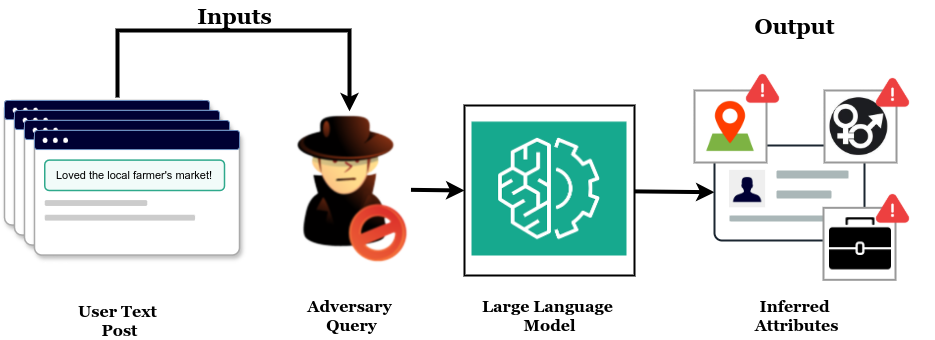
\includegraphics[width=\columnwidth]{figures/llm_inference_attack_pipeline.png}
\caption{UAL-Inference attack pipeline. The attacker pairs the victim's text with a profiling query; the target LLM processes both jointly and returns inferred attributes (location, gender, occupation, and other privacy-sensitive fields) that were never explicitly stated in the source text.}
\label{fig:threat_pipeline}
\end{figure}

The attacker's capabilities are limited to the standard text interface exposed to any user of the target LLM. The attacker has no access to model weights, gradients, activations, or training data, and mounts the entire attack through ordinary prompting; the only capability required is the ability to submit an arbitrary natural-language query alongside the victim's text and to freely reformulate that query, including through paraphrase, role-play framing, indirect phrasing, or conversational misdirection, in order to evade a defense positioned at the input boundary. In terms of knowledge and access, the attacker is assumed to already possess the target document UAL-Inference is not a data-exfiltration attack and does not, by itself, grant access to text the attacker does not already have and requires no auxiliary side-channel information about the victim beyond that document; the attacker interacts with the system through the same interface as a legitimate user and is, at the transport layer, indistinguishable from one.

Figure~\ref{fig:threat_pipeline} illustrates the resulting attack pipeline: the victim's text and the attacker's query are jointly submitted to the target LLM, which returns a structured estimate of the victim's attributes each carrying an associated privacy risk, illustrated in the figure by attributes such as location, gender, and occupation. In practice, the attacker's query ranges from an explicit profiling command to a superficially benign analytical request (e.g., framed as summarization or opinion analysis) that preserves the same underlying objective while avoiding syntactic markers a naive filter might key on; Section~\ref{sec:methodology} operationalizes this range as nine concrete prompt variants spanning the explicit-to-evasive spectrum introduced in Section~\ref{subsec:two_axes}.

The target LLM itself is treated as a black box that is assumed to process attribute-profiling requests unless they are intercepted by a defense positioned at the input boundary; the model is not assumed to be adversarially modified or fine-tuned by the attacker. Weight-level interventions such as safety fine-tuning or RLHF alignment, post-generation output filters, and multi-turn attacks that split a profiling request across several conversational turns are outside the scope of the threat model
considered here; the latter is discussed as a limitation in
Section~\ref{sec:discussion}.

\subsection{Defense Requirements}
\label{subsec:defense_requirements}

This threat model directly determines what a defense must satisfy to be effective. First, because the attacker's objective is defined by the semantic purpose of the request rather than by any particular wording, a defense restricted to syntactic or lexical pattern matching cannot reliably separate UAL-Inference from benign analytical tasks; detection must instead operate on the semantic relation expressed by the query whether it asks the model to infer a private attribute of the person represented by the supplied text which is the central design principle behind UAL Semantic Guard.

Second, since the threat model grants the attacker unrestricted reformulation of the query, a defense must remain effective across paraphrase, indirect phrasing, role-play framing, and other surface-level rewrites that preserve the same underlying profiling intent; a mechanism that only recognizes the specific phrasings it was designed or trained against fails against this capability by construction, motivating the evasive attack variants used in our evaluation.

Third, a defense that satisfies these two properties is still unfit for deployment if it is not also conservative on legitimate traffic: because ordinary analytical tasks such as summarization, translation, or sentiment analysis can superficially resemble a profiling request, a defense must keep its false-positive rate low enough not to degrade the very use cases that motivate deploying an LLM in the first place, which we treat as a first-class evaluation axis alongside detection rate.

Finally, because the defense sits on the critical path of every request, it must add an acceptable latency and energy overhead per query to be practically deployable at scale; this operational cost is not a secondary concern but a direct deployment constraint, which is why Section~\ref{sec:results} reports inference latency and energy consumption with the same rigor as detection and false-positive rates.
